\section{Objetivos}
\subsection{Objetivo General}

Explorar las interacciones entre genes y proteínas asociadas al Signo de Hoffman, utilizando bases de datos bioinformáticas y herramientas de análisis de redes para identificar posibles grupos funcionales y patrones de interacción relevantes.

\subsection{Objetivos Específicos}
\begin{enumerate}
	\item Identificar genes asociados al signo de Hoffman mediante la utilización de la Human Phenotype Ontology (HPO) y otras bases de datos relevantes.
	\item Construir una red de interacciones proteína-proteína (PPI) basada en los genes obtenidos, utilizando StringDB para analizar las interacciones de las proteínas codificadas por estos genes.
	\item Aplicar algoritmos de análisis de redes, como iGraph, para calcular métricas topológicas y determinar características clave de la red.
	\item Aplicar clustering en la red de interacción para identificar grupos de genes o proteínas que presenten una alta conectividad.
	\item Determinar las principales funciones biológicas y vías metabólicas en las que están involucrados los genes identificados mediante enriquecimiento funcional.
\end{enumerate}

\section{Materiales y Herramientas}

A continuación, se detalla cada uno de los materiales empleados para la realización de este trabajo.

\subsection{Bases de datos}

\subsubsection{Human Phenotype Ontology (HPO)}
  Es una base de datos que estandariza los fenotipos clínicos humanos y vincula genes y enfermedades a cada fenotipo obteniendo las interacciones genéticas.\cite{gargano2024}. 
\subsubsection{StringDB}
La base de datos STRING (\textit{Search Tool for the Retrieval of Interacting Genes/Proteins}) es una base de datos que reúne datos experimentales, predicciones y literatura para informar sobre interacciones proteicas. \cite{szklarczyk2019}.

\subsection{Lenguajes de Programación}

\subsubsection{R}
El lenguaje de programación \textit{R} específicamente la versión 4.3.3. Es un lenguaje para exploración estadística y creación de gráficos. Es flexible, ampliable con paquetes y de código abierto bajo el proyecto GNU. \cite{chan2018}.


\paragraph{Manipulación y Visualización de Datos:}
\begin{itemize}
	\item \textbf{tidyverse}: Conjunto de paquetes (incluyendo \textit{dplyr} y \textit{ggplot2}) que permiten manipular y graficar datos. \textit{dplyr} facilita el manejo de grandes datasets, mientras que \textit{ggplot2} permite generar gráficos de alta calidad \cite{Wickham2019}.
\end{itemize}

\paragraph{Análisis Bioinformático:}
\begin{itemize}
	\item \textbf{Bioconductor}: Conjunto de paquetes especializados en el análisis de datos genómicos. \cite{Huber2015}.
	\item \textbf{iGraph para R}: Versión de iGraph en R, útil para la comparación de redes de interacción generadas en Python y el análisis estadístico de propiedades de red. \cite{Csardi2006}.
\end{itemize}


\subsubsection{Python}
El lenguaje de programación \textit{Python} es versátil y de alto nivel, usado en diversas aplicaciones.  Es interpretado, por lo que no requiere compilación previa, que permite el uso de librerías y APIs para diversas funciones. A continuación, se describen las librerías específicas empleadas en este estudio:

\paragraph{Análisis de Redes y Grafos:}
\begin{itemize}
	\item \textbf{iGraph}: Capaz de calcular métricas topológicas, análisis de comunidades y otras manipulaciones de redes complejas \cite{igraph2006}.
	\item \textbf{NetworkX}: Complemento de iGraph para la visualización y análisis interactivo de grafos, permitiendo inspeccionar la estructura y propiedades de redes de interacción proteína-proteína (PPI) \cite{hagberg2008}.
\end{itemize}

\paragraph{Visualización de Datos:}
\begin{itemize}
	\item \textbf{Matplotlib}: Proporciona las bases para crear gráficos y representaciones visuales básicas en Python, útil en la representación gráfica de resultados bioinformáticos \cite{Hunter2007}.
	\item \textbf{Seaborn}: Ofrece una visualización de datos avanzada y estilizada, ideal para gráficos estadísticos que ayudan a visualizar las propiedades estructurales de redes y distribuciones de datos \cite{Waskom2021}.
\end{itemize}

\paragraph{Extracción y Manipulación de Datos:}
\begin{itemize}
	\item \textbf{Requests}: Necesario para realizar consultas a APIs como HPO y StringDB, a fin de recuperar datos de interacciones. \cite{Requests2020}.
	\item \textbf{Pandas}: Herramienta de manipulación de datos, utilizada para estructurar y limpiar datos previos a su análisis en redes.\cite{McKinney2010}.
\end{itemize}




\subsection{Software y Herramientas Computacionales}

\subsubsection{Entornos de Programación y Computación}
Para el desarrollo de los scripts y la ejecución de los análisis, existen editores de texto como \textit{Visual Studio Code} y \textit{RStudio} para escribir y depurar el código en Python y R, respectivamente. Ambos entornos ofrecen características avanzadas de edición.

\subsubsection{GitHub}
Para el control de versiones y la gestión de código  existen plataformas como \textit{GitHub}. Que permite gestionar los scripts de Python y R, así como los datos intermedios generados durante el análisis. GitHub es una plataforma de desarrollo colaborativo de software que permite a los usuarios almacenar, compartir y gestionar proyectos de código abierto.\cite{dozmorov2018}. 


\subsection{Algoritmos de Análisis}

Para evaluar las redes de interacción obtenidas y realizar el análisis de agrupamiento, se utilizaron diversas variaciones de algoritmos conocidos:
\\

\begin{itemize}
	\item \textbf{Algoritmo de Clustering (Louvain)}: Este algoritmo optimiza la partición de una red maximizando su modularidad, lo cual es especialmente útil en redes grandes y complejas. Es ampliamente utilizado para detectar comunidades en redes biológicas, proporcionando un análisis modular efectivo de interacciones genéticas \cite{Blondel2008}.
	
	\item \textbf{DIAMOnD}: (A DIseAse MOdule Detection) identifica módulos de enfermedades en redes de interacción proteína-proteína al expandir conjuntos de genes conocidos con nodos topológicamente cercanos. Aunque prioriza bien genes asociados a enfermedades, su eficacia disminuye con grandes volúmenes de genes candidatos.\cite{Ghiassian2015}.
	
	\item \textbf{Propagación de Etiquetas}: Este algoritmo agrupa datos según su similitud, sin la necesidad de especificar el número de clústeres a priori, haciéndolo adecuado para una exploración inicial de la estructura de la red \cite{Raghavan2007}.
	
	\item \textbf{Métricas de Análisis de Redes}: Para caracterizar las propiedades estructurales de las redes generadas, se emplearon métricas como la centralidad de grado, el coeficiente de agrupamiento y la centralidad de intermediación. Estas métricas permiten comprender cómo los genes o proteínas se conectan entre sí dentro de la red y resaltar los nodos más relevantes en términos biológicos.
	
	\item \textbf{Enriquecimiento Funcional}: Una vez identificados los clusters, se realizó un análisis de enriquecimiento funcional para determinar qué funciones biológicas, rutas metabólicas o procesos celulares están sobrerrepresentados en los grupos de genes o proteínas detectados. 
\end{itemize}



\section{Métodos}

\subsection{Flujo de trabajo}

\begin{figure}[h!]
	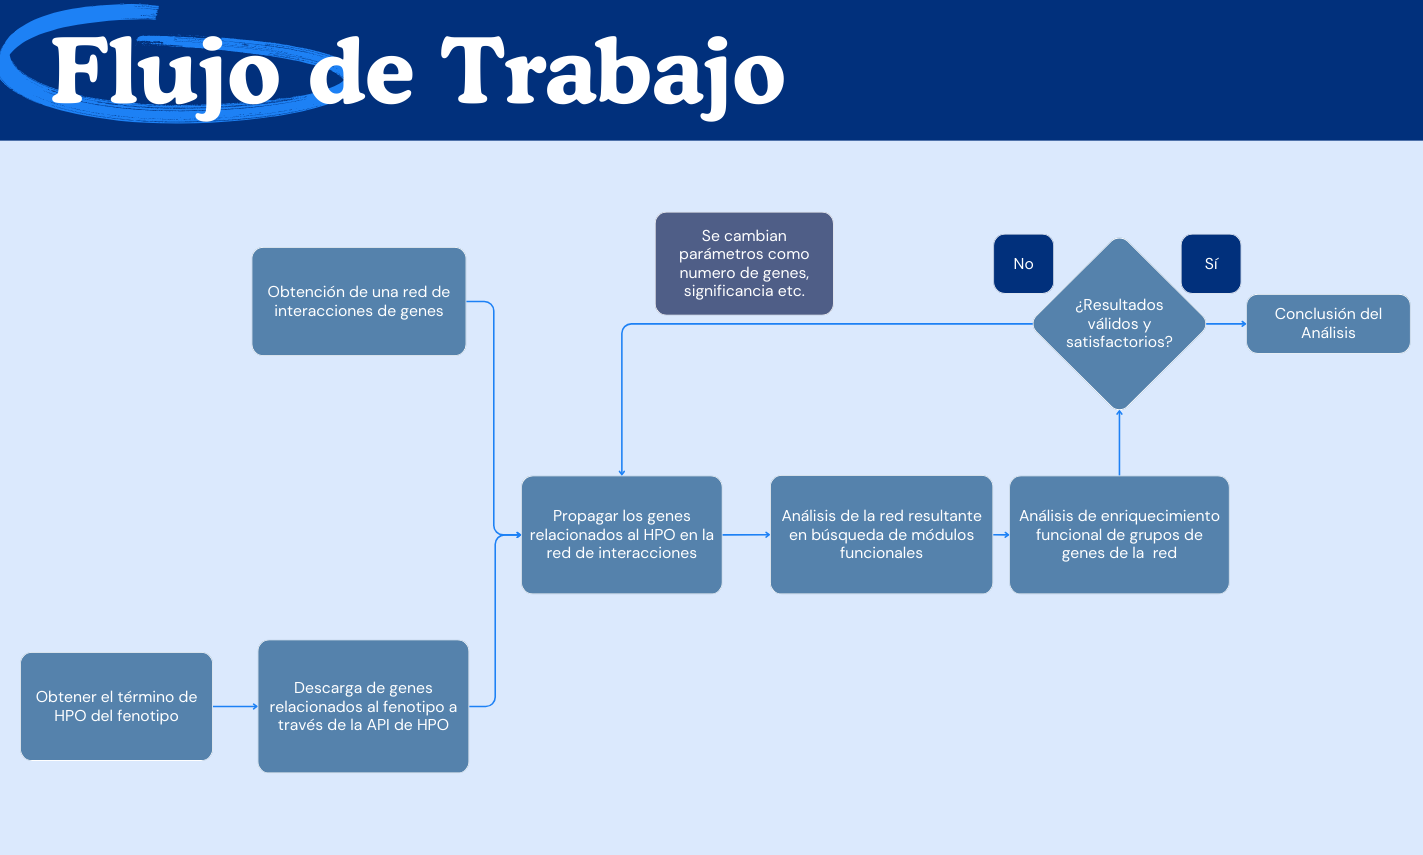
\includegraphics[width=.95\textwidth]{figures/workflow.png}
	\caption{Flujo de trabajo}
	\label{fig:workflow}
\end{figure}

\subsection{Obtención de genes relacionados con signo de Hoffman}

Para obtener los genes relacionados con el signo de Hoffman (HP:0031993), se utilizó la API de la Ontología de Fenotipos Humanos (HPO). En este caso, se emplearon endpoints de la API que devuelven listas tanto de genes (\url{https://ontology.jax.org/api/network/annotation/HP:0031993/download/gene}) como de enfermedades vinculadas al fenotipo de interés (\url{https://ontology.jax.org/api/network/annotation/HP:0031993/download/disease}). Mediante una solicitud HTTP, se extrajo y almacenó esta información en archivos con formato .tsv, facilitando así su posterior análisis. 


\subsection{Obtención de red de interacciones de genes}

Para el análisis de las interacciones génicas, se obtuvo una red de interacciones a partir de la base de datos STRING.

El archivo correspondiente a las interacciones de proteínas humanas (\textit{Homo sapiens}, ID taxonómico: 9606) fue descargado directamente desde \href{https://stringdb-downloads.org/download/protein.links.v12.0/9606.protein.links.v12.0.txt.gz}{el repositorio público de STRING} utilizando un comando en la consola.

Posteriormente, las interacciones fueron filtradas aplicando un umbral mínimo de puntuación combinada (\textit{combined score}) de 700. Posteriormente los identificadores de las proteínas se transformaron a identificadores estándar HUGO.

\subsection{Propagación de red}

Se utilizó el algoritmo DIAMOnD para expandir genes relacionados con el signo de Hoffman en la red de interacciones proteína-proteína. El algoritmo parte de un conjunto inicial de genes de semilla, identificando nodos adicionales cercanos en términos de proximidad topológica, evaluando su conectividad mediante una distribución hipergeométrica. La selección de nodos se basa en su número de conexiones con los genes de semilla, priorizando aquellos que forman una subred coherente, en el proceso biológico del signo de Hoffman. Lo que resultó en una red enriquecida de genes candidatos, visualizados como una subred relacionada con el fenotipo.

\subsection{Análisis de red}
Se aplicó el algoritmo de Louvain para identificar módulos funcionales en la red, agrupando nodos en función de la densidad de sus interacciones. Posteriormente, se calcularon métricas topológicas para analizar la estructura y el rol de los genes en la red. La centralidad de grado permitió identificar nodos con alta conectividad dentro de sus módulos, mientras que la centralidad de intermediación destacó los genes clave en el flujo de información entre módulos. Por último, la centralidad de cercanía ayudó a identificar nodos importantes para la cohesión interna de los módulos.

Este análisis facilitó la identificación de módulos funcionales representados por grupos de genes con posibles relaciones biológicas.

\subsection{Análisis de enriquecimiento funcional}

Una vez identificados los clusters, se realizó un análisis de enriquecimiento funcional para determinar qué funciones biológicas, rutas metabólicas o procesos celulares están sobrerrepresentados en los grupos de genes detectados.